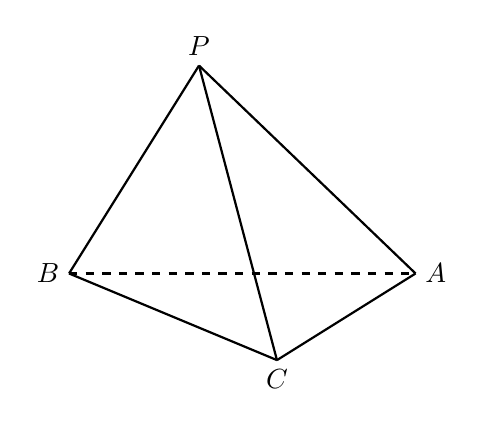
\begin{tikzpicture}[scale=1.1,>=stealth]
  % 顶点坐标
  \coordinate (P) at (1.5, 3.2);
  \coordinate (B) at (0, 0.8);
  \coordinate (A) at (4.0, 0.8);
  \coordinate (C) at (2.4, -0.2);

  % 棱
  \draw[thick] (P) -- (B);
  \draw[thick] (P) -- (C);
  \draw[thick] (P) -- (A);
  \draw[thick] (B) -- (C);
  \draw[thick] (C) -- (A);
  \draw[dashed, thick] (B) -- (A);

  % 顶点标注
  \node[above] at (P) {$P$};
  \node[left] at (B) {$B$};
  \node[below] at (C) {$C$};
  \node[right] at (A) {$A$};
\end{tikzpicture}
